\documentclass{beamer}
\usetheme{Boadilla}
\usepackage{captdef}
\usepackage{tikz}
\usetikzlibrary{shapes.geometric, arrows}
\tikzstyle{arrow} = [thick,->,>=stealth]
\usepackage{listings}
\usepackage{subfigure} % For subfigures
\usepackage{verbatim}
\usepackage{tikz}
\usetikzlibrary{shapes.geometric, arrows}
\tikzstyle{startstop} = [rectangle, rounded corners, minimum width=3cm, minimum height=1cm,text centered, draw=black, fill=red!30]
\tikzstyle{io} = [trapezium, trapezium left angle=70, trapezium right angle=110, minimum width=3cm, minimum height=1cm, text centered, draw=black, fill=blue!30]
\tikzstyle{process} = [rectangle, minimum width=3cm, minimum height=1cm, text centered, draw=black, fill=orange!30]
\tikzstyle{decision} = [diamond, minimum width=3cm, minimum height=1cm, text centered, draw=black, fill=green!30]
\tikzstyle{arrow} = [thick,->,>=stealth]

%just to simplifly the body of the document
\newcommand\img[1]{%
\centering
\includegraphics[width=\linewidth, height=.4\textheight]%
{#1}
%\par\figcaption{Caption of \MakeUppercase #1}
}


%Information to be included in the title page:
\title{Summary 1st day}
\subtitle{Model building}
%\author{R. Marabini}
%\institute{EPS-UAM}
\date{}

\begin{document}

\frame{\titlepage}

\begin{frame}
\LARGE
\frametitle{Objective}

To \textbf{construct 3D atomic models} of biomolecules (typically proteins) based on experimental or predicted data, enabling insights into their \textbf{function}.

\end{frame}


\begin{frame}
\LARGE
\frametitle{1st step: Map Preprocessing.-  enhance map sharpness}

One effective approach is local filtering (LocalDeblur), which adaptively enhance features based on local resolution.

\end{frame}

\begin{frame}
\LARGE
\frametitle{2nd step: Initial Model}
\begin{itemize}
 \item Alphafold
    \begin{itemize}
    \item Highly accurate, especially for single-chain proteins (5000)
    \item No experimental structure is used
    \item Main input sequences
    \item Relies on coevolution
    \end{itemize}
 \item ModelAngelo
    \begin{itemize}
    \item Integrates structural constraints (3D maps)
    \item Works better at resolution less than 3.5 \AA
    \end{itemize}
 \item  Modeller (Sequence Homology Modeling)
    \begin{itemize}
    \item Builds models based on known structures of similar sequences
    \item Relies on evolutionary conservation
    \item Effective when homologous templates are available
    \end{itemize}
\end{itemize}
\end{frame}


\LARGE
\title{Summary 2nd day}
\subtitle{Model building}
\frame{\titlepage}

\begin{frame}
\frametitle{Workflow}
\center
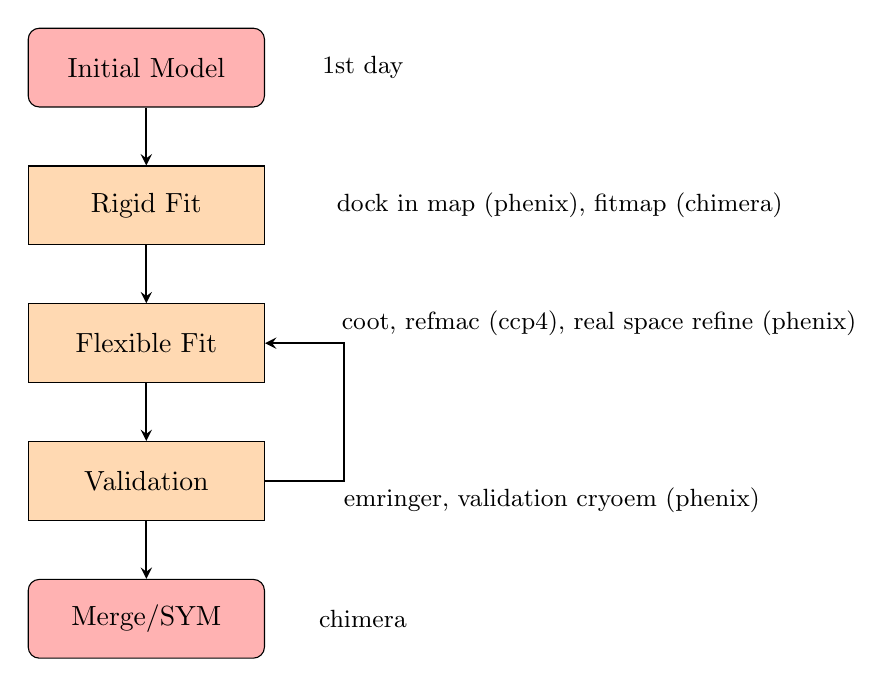
\begin{tikzpicture}[node distance=1.75cm]
    \node (initialmodel) [startstop] {Initial Model};
    \node (rigidfit) [process, below of=initialmodel] {Rigid Fit};
    \node (flexiblefit) [process, below of=rigidfit] {Flexible Fit};
    \node (validation) [process, below of=flexiblefit] {Validation};
    \node (mergesym) [startstop, below of=validation] {Merge/SYM};

    %\node (dec1) [decision, right of=validation] {Decision 1};


    \draw [arrow] (initialmodel) -- (rigidfit);
    \draw [arrow] (rigidfit) -- (flexiblefit);
    \draw [arrow] (flexiblefit) -- (validation);
    \draw [arrow] (validation) -- (mergesym);

    \draw [arrow] (validation.east) to node[anchor=north] {} ++(0:1) |- (flexiblefit.east);


    \node(initialmodel_text)[right of=initialmodel, xshift=1cm] {\small 1st day};
    \node(rigidfit_text)[right of=rigidfit, xshift=3.5cm] {\small dock in map (phenix), fitmap (chimera)};
    \node(flexiblefit_text)[right of=flexiblefit, xshift=4.0cm, yshift=0.25cm] {\small coot, refmac (ccp4), real space refine (phenix)};
    \node(validation_text)[right of=validation, xshift=3.4cm, yshift=-0.25cm] {\small emringer, validation cryoem (phenix)};
    \node(mergesym_text)[right of=mergesym, xshift=1cm] {\small chimera};

\end{tikzpicture}

\end{frame}


\begin{comment}


\begin{frame}{Descripción de la aplicación: Proceso electoral}
    \centering
    \begin{figure}
         \subfigure[\tiny Existe un censo (modelo ``Censo'' en models.py)]{\includegraphics[width=0.45\textwidth, height=0.3\textheight]{images/censo0.jpg}}
         \subfigure[\tiny Mediante el formulario ``CensoForm'' y la vista ``aportarinfo\_censo'' se verifican los datos]
         {\includegraphics[width=0.45\textwidth, height=0.3\textheight]{images/censo-verifica.jpg}} \\
         \subfigure[\tiny Se vota (VotoForm-aportarinfo\_voto)]{\includegraphics[width=0.45\textwidth, height=0.3\textheight]{images/voto.jpg}}
         \subfigure[\tiny utils (list-getvotos-/delete-delvoto-/create-testdb-)]{\includegraphics[width=0.45\textwidth, height=0.3\textheight]{images/utils.png}}
     \end{figure}
\end{frame}

\begin{frame}
\frametitle{Desacoplar Servidor y cliente - I (P1-base)}
    \begin{figure}
        \centering
        \includegraphics[width=0.8\textwidth]{images/back-front-1.png}
        %\caption{Desplegar código en las MV usando git}
    \end{figure}
\end{frame}

\begin{frame}
\frametitle{Desacoplar Servidor y cliente - II}
    \begin{figure}
        \centering
        \includegraphics[width=0.8\textwidth]{images/back-front-2.jpg}
        % \caption{API }
    \end{figure}
\end{frame}



\begin{frame}
\frametitle{Backend-Frontend (SI2)}
\tikzstyle{startstop} = [rectangle, rounded corners, minimum width=3cm, minimum height=1cm,text centered, draw=black, fill=red!30]
\centering
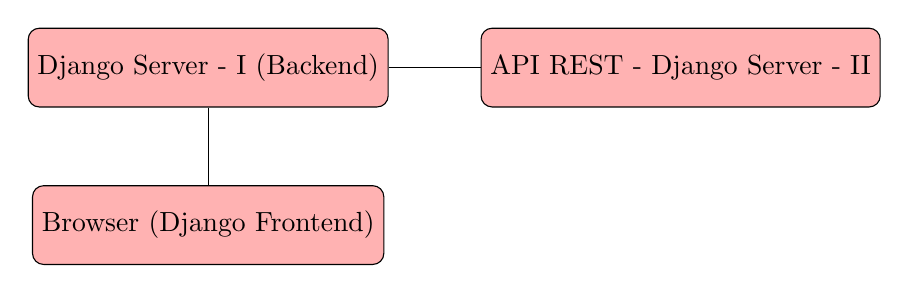
\begin{tikzpicture}[node distance=2cm]
    \node (vuejs) [startstop] {Django Server - I (Backend)};
    \node (serve) [startstop, below of=vuejs] {Browser (Django Frontend)};
    %\node (browser) [startstop, below of=serve] {Browser};
    \node (apirest) [startstop, right of=vuejs, xshift=4cm] {API REST - Django Server - II};

    \draw [] (vuejs) -- node[anchor=east] {} (serve);
    %\draw [arrow] (serve) -- node[anchor=east] {} (browser);

    \draw [] (vuejs) -- node[anchor=south] {} (apirest); % Path with a label above

\end{tikzpicture}

\end{frame}


\begin{frame}
\frametitle{Backend-Frontend (PSI)}
\tikzstyle{startstop} = [rectangle, rounded corners, minimum width=3cm, minimum height=1cm,text centered, draw=black, fill=red!30]
\centering
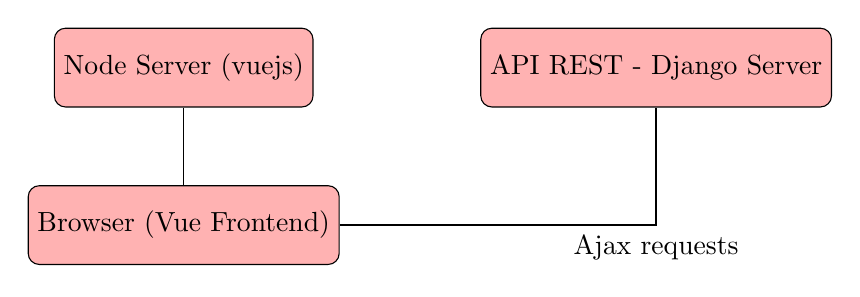
\begin{tikzpicture}[node distance=2cm]
    \node (vuejs) [startstop] {Node Server (vuejs)};
    \node (serve) [startstop, below of=vuejs] {Browser (Vue Frontend)};
    \node (apirest) [startstop, right of=vuejs, xshift=4cm] {API REST - Django Server};

    \draw[] (vuejs) -- node[anchor=east] {} (serve);

    \draw[thick] (serve) -| node[below] {Ajax requests} (apirest); % Path with a label above

\end{tikzpicture}

\end{frame}


\begin{frame}{API REST: Aplicación web tradicional}
    \begin{figure}
        \centering
        \includegraphics[width=0.8\textwidth]{images/api01.png}
    \end{figure}
    \begin{itemize}
    \footnotesize
     \item El cliente debe entender HTML.
     \item Las páginas se repintan en cada llamada.
     \item El mismo código se envía múltiple veces (p.e. ficheros de estilo).
    \end{itemize}

\end{frame}

\begin{frame}{API REST}
    \begin{figure}
        \centering
        \includegraphics[width=0.8\textwidth]{images/api02.png}
    \end{figure}
\end{frame}


\begin{frame}{Convenciones seguidas por el API REST}
\begin{itemize}
 \item Usa URIs para identificar los recursos (htttp://host/\textbf{votos})
 \item Usa métodos HTTP para especificar la operación
     \begin{itemize}
      \item POST (crear)
      \item GET (operaciones de solo lectura como listados)
      \item PUT (actualizar)
      \item DELETE (borrar)
     \end{itemize}
\item Usa el cabecero HTTP para especificar el formato de intercambio de datos(p.e. JSON)
\item Usa los códigos HTTP para indicar el éxito o fracaso de la petición (200 -OK-, 201 -CREATED-, etc)

\end{itemize}

\end{frame}

\begin{frame}{API REST}
    \begin{figure}
        \centering
        \begin{figure}
         %\pause\subfigure[\tiny Existe un censo (modelo ``Censo'' en models.py]
        \includegraphics[width=0.8\textwidth]{images/api04.png}
        \includegraphics[width=0.8\textwidth]{images/api05.png}
        \end{figure}

        \end{figure}
\end{frame}




\begin{frame}
\frametitle{Publicar código en las máquinas virtuales}
    \begin{figure}
        \centering
        \includegraphics[width=0.8\textwidth]{images/git_remote.pdf}
    \end{figure}
\end{frame}

\begin{frame}
\frametitle{``push'' no actualiza el código}
    \begin{figure}
        \centering
        \includegraphics[width=0.5\textwidth]{images/deploy-project-with-git.png}
    \end{figure}

\end{frame}

\begin{frame}[fragile]
\frametitle{Git ``hooks''}
Edita:

\begin{lstlisting}
# VM2
nano /home/si2/repo/p1base.git/hooks/post-receive
\end{lstlisting}

    Agrega las siguientes líneas al archivo:
\begin{lstlisting}
#!/bin/bash
GIT_WORK_TREE=/home/si2/repo/p1base git checkout -f
\end{lstlisting}
%    Si el directorio \texttt{/home/si2/repo/p1base} no existe créalo. Esta será la ubicación del directorio de trabajo.

%     Haz que el archivo sea ejecutable:
%\begin{minted}{python}
%chmod +x /home/si2/repo/p1base.git/hooks/post-receive
%    \end{minted}


\end{frame}
\end{comment}


\end{document}
